
\section{Reference preview slope nélkül}

 
 Az alább látható szabályzók már ismerték a zavarjel értékát 2.5 órával előre. A referenciajelet konstansnak állítottam be.
 
 Állandósult állapotban 10 napos mintákat ábrázoltam, és ezeket feldolgozva numerikusan is összehasonlítottam a szabályozókat.
 A külső hőmérséklet értéket egy négyszögjel felfutási idejének korlátozásával kaptam.
 
 Különböző költségfüggvényű MPC-k más-más arányban használták a beavatkozókat és más-más mértékben tértek el az alapjeltől. Az összesítésben leolvashatók ezek az arányok.
 
\begin{figure}[H]
	\centering
	% trim={<left> <lower> <right> <upper>}
	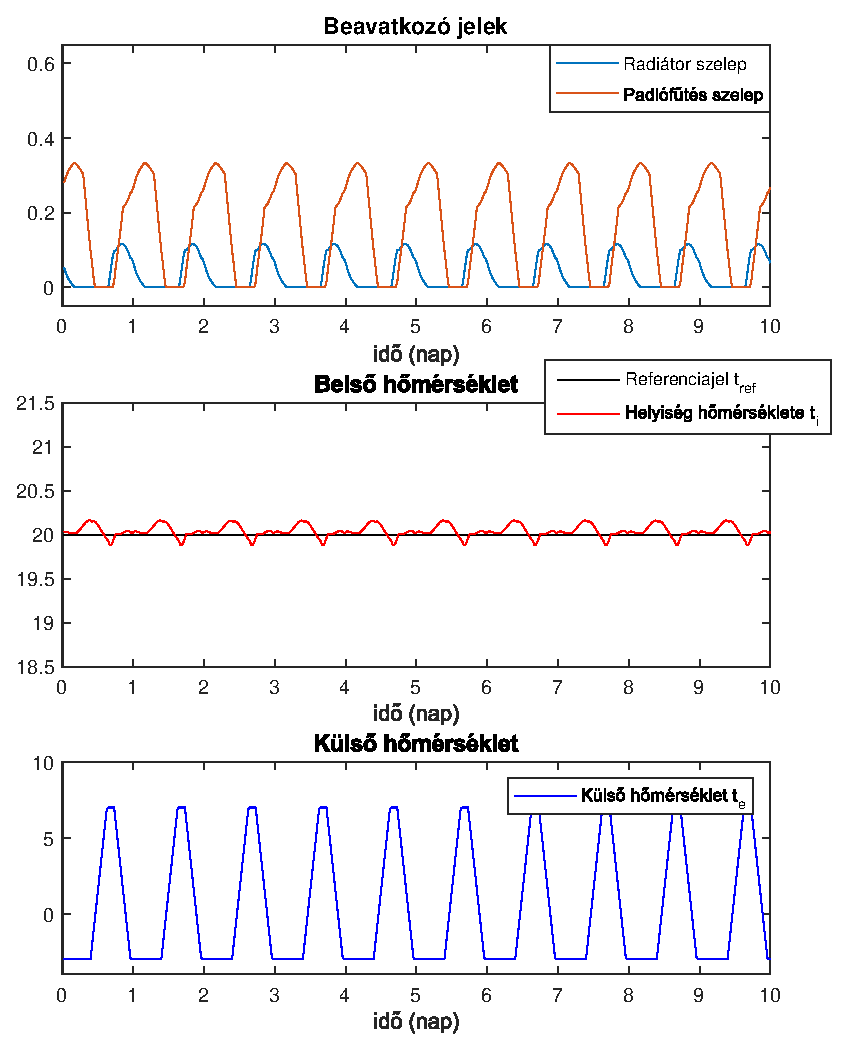
\includegraphics[width=0.35\textwidth, trim=0 0 0 0, clip,]{figures/onlab/NoSlope/CLast10ClosedLoop}
	\caption{Referenciajel figyelembe vétele a teljes horizontra CLast10ClosedLoop}
	\label{fig:onlab-refprev1}
\end{figure}

\begin{figure}[H]
\centering
% trim={<left> <lower> <right> <upper>}
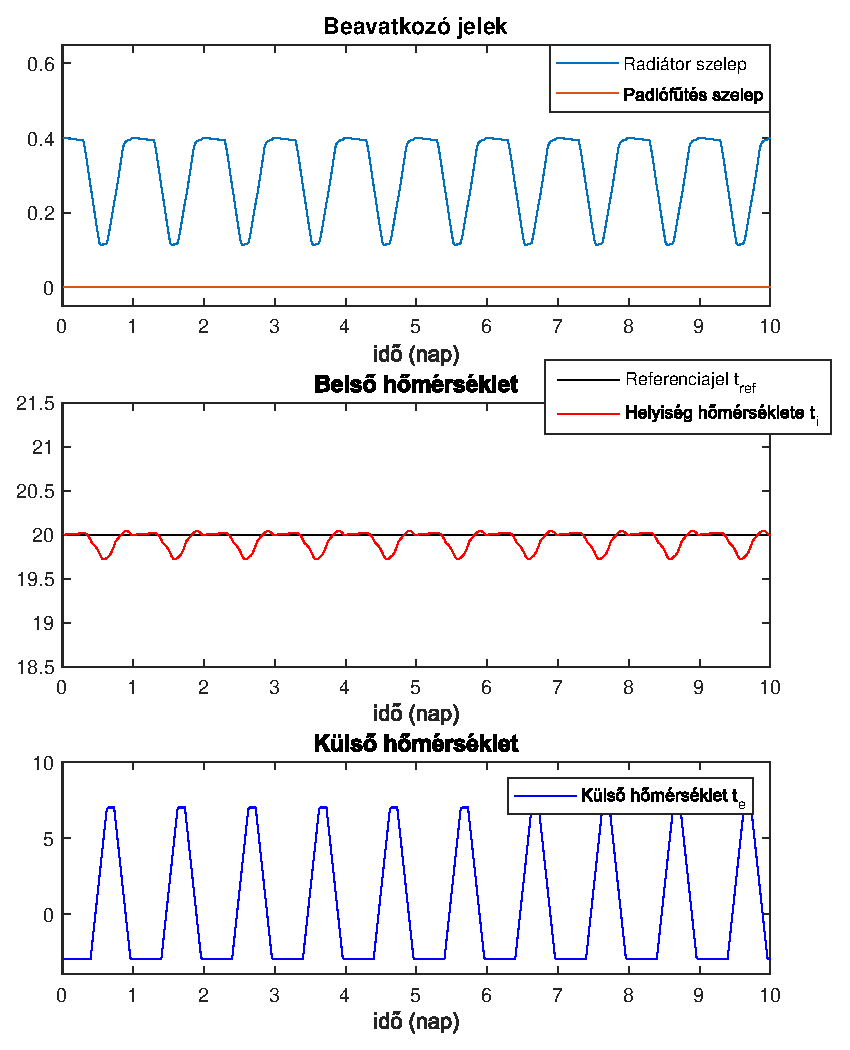
\includegraphics[width=0.35\textwidth, trim=0 0 0 0, clip,]{figures/onlab/NoSlope/C1Last10ClosedLoop}
\caption{Referenciajel figyelembe vétele a teljes horizontra C1Last10ClosedLoop}
\label{fig:onlab-refprev2}
\end{figure}

\begin{figure}[H]
\centering
% trim={<left> <lower> <right> <upper>}
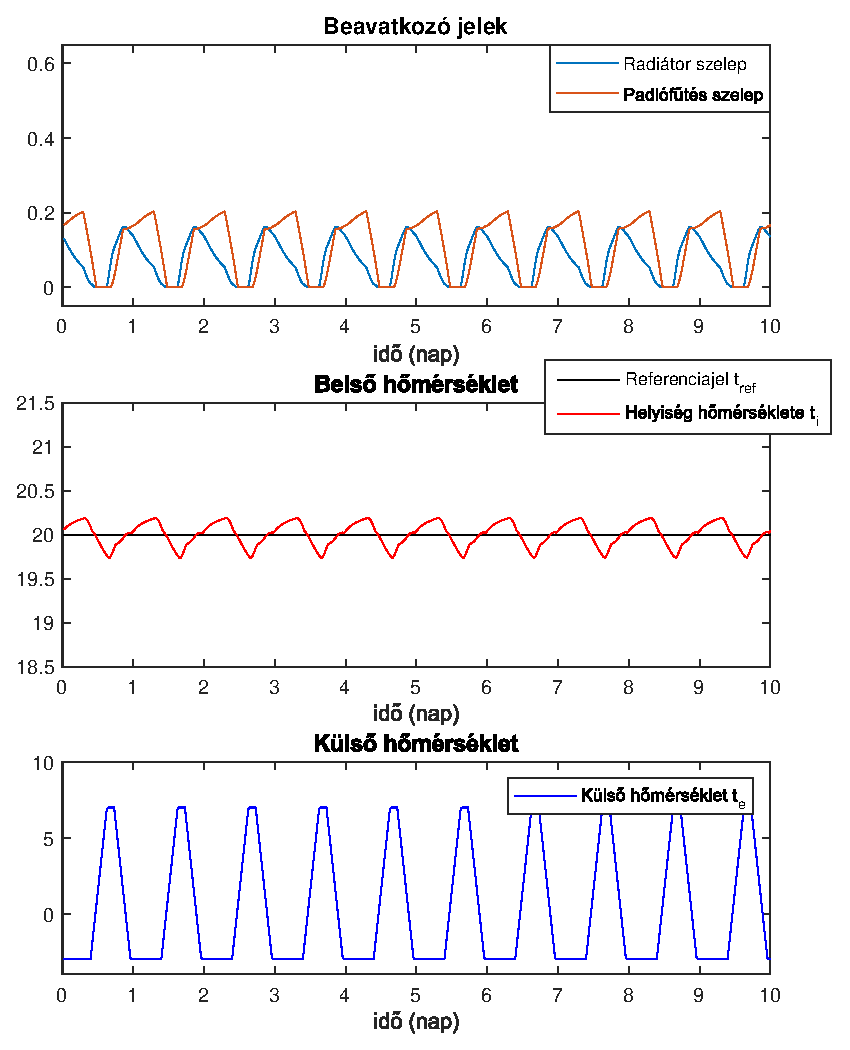
\includegraphics[width=0.35\textwidth, trim=0 0 0 0, clip,]{figures/onlab/NoSlope/C2Last10ClosedLoop}
\caption{Referenciajel figyelembe vétele a teljes horizontra C2Last10ClosedLoop}
\label{fig:onlab-refprev3}
\end{figure}

\begin{figure}[H]
\centering
% trim={<left> <lower> <right> <upper>}
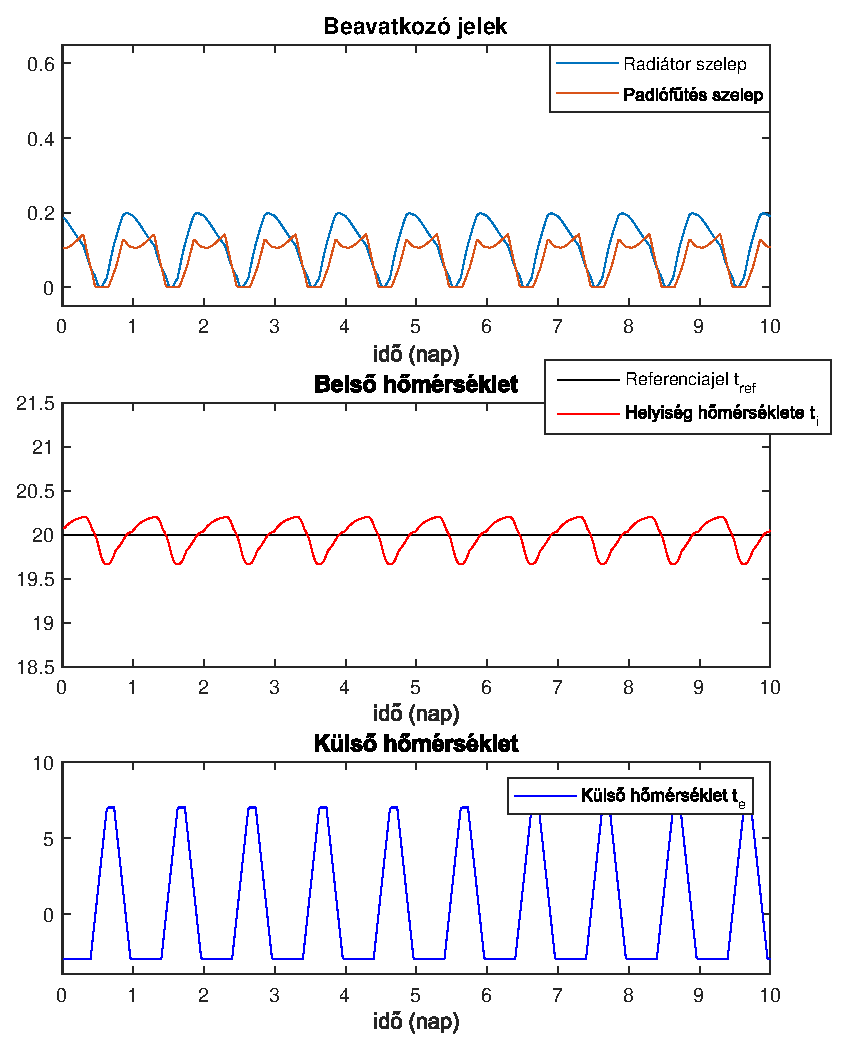
\includegraphics[width=0.35\textwidth, trim=0 0 0 0, clip,]{figures/onlab/NoSlope/C4Last10ClosedLoop}
\caption{Referenciajel figyelembe vétele a teljes horizontra C4Last10ClosedLoop}
\label{fig:onlab-refprev4}
\end{figure}

\begin{figure}[H]
\centering
% trim={<left> <lower> <right> <upper>}
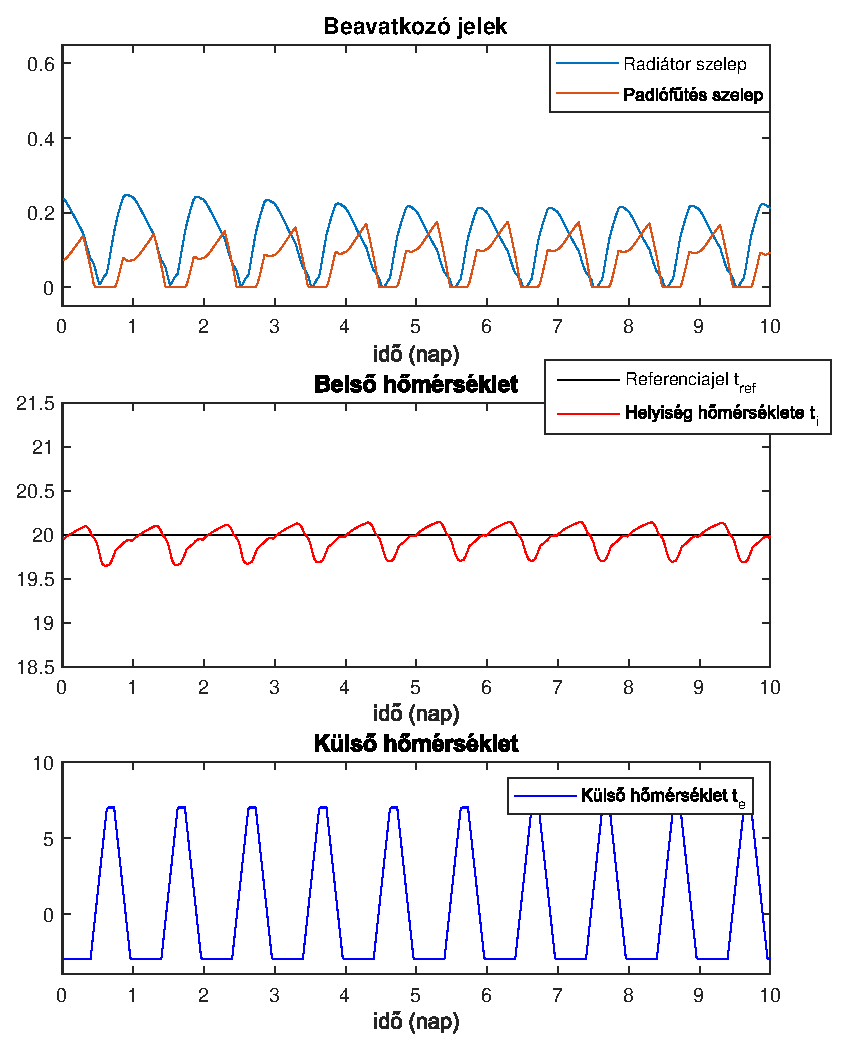
\includegraphics[width=0.35\textwidth, trim=0 0 0 0, clip,]{figures/onlab/NoSlope/C5Last10ClosedLoop}
\caption{Referenciajel figyelembe vétele a teljes horizontra C5Last10ClosedLoop}
\label{fig:onlab-refprev5}
\end{figure}

\subsection{Összehasonlítás}
\begin{figure}[H]
	\centering
	% trim={<left> <lower> <right> <upper>}
	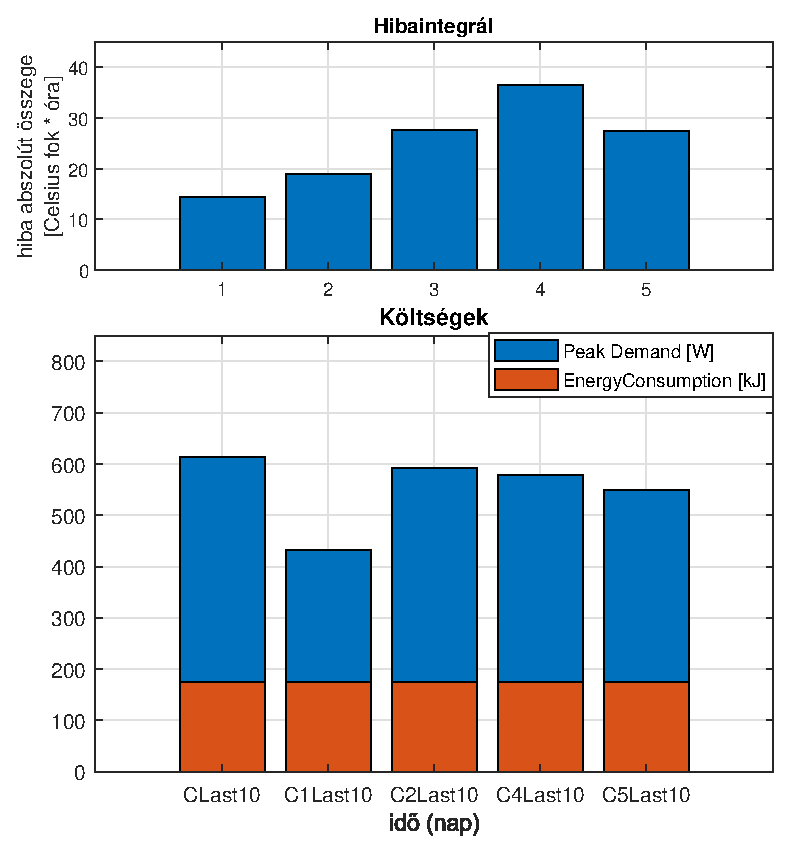
\includegraphics[width=0.35\textwidth, trim=0 0 0 0, clip,]{figures/onlab/NoSlope/compareControllerJustPreview}
	\caption{compareControllerJustPreview}
	\label{fig:onlab-refprevComp}
\end{figure}

\pagebreak


\section{Reference preview slopepal}

\begin{figure}[H]
	\centering
	% trim={<left> <lower> <right> <upper>}
	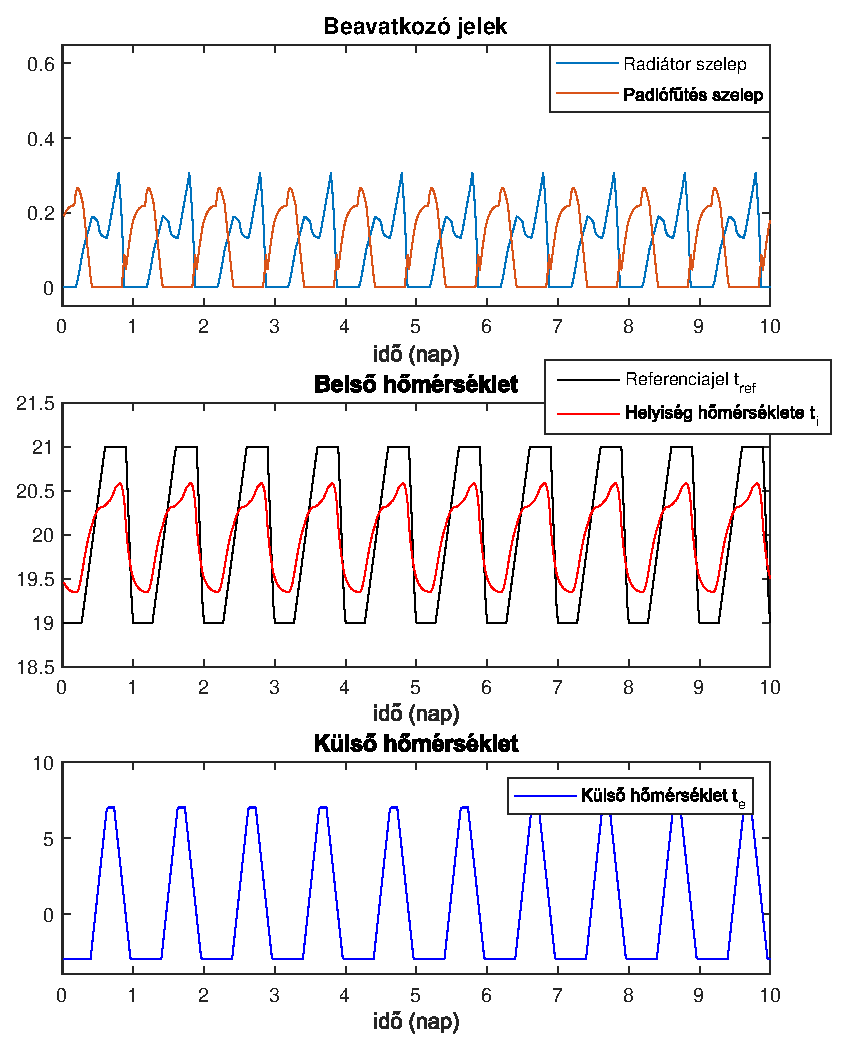
\includegraphics[width=0.35\textwidth, trim=0 0 0 0, clip,]{figures/onlab/Slope/CLast10ClosedLoop}
	\caption{Referenciajel figyelembe vétele a teljes horizontra CLast10ClosedLoop}
	\label{fig:onlab-refslprev}
\end{figure}

\begin{figure}[H]
	\centering
	% trim={<left> <lower> <right> <upper>}
	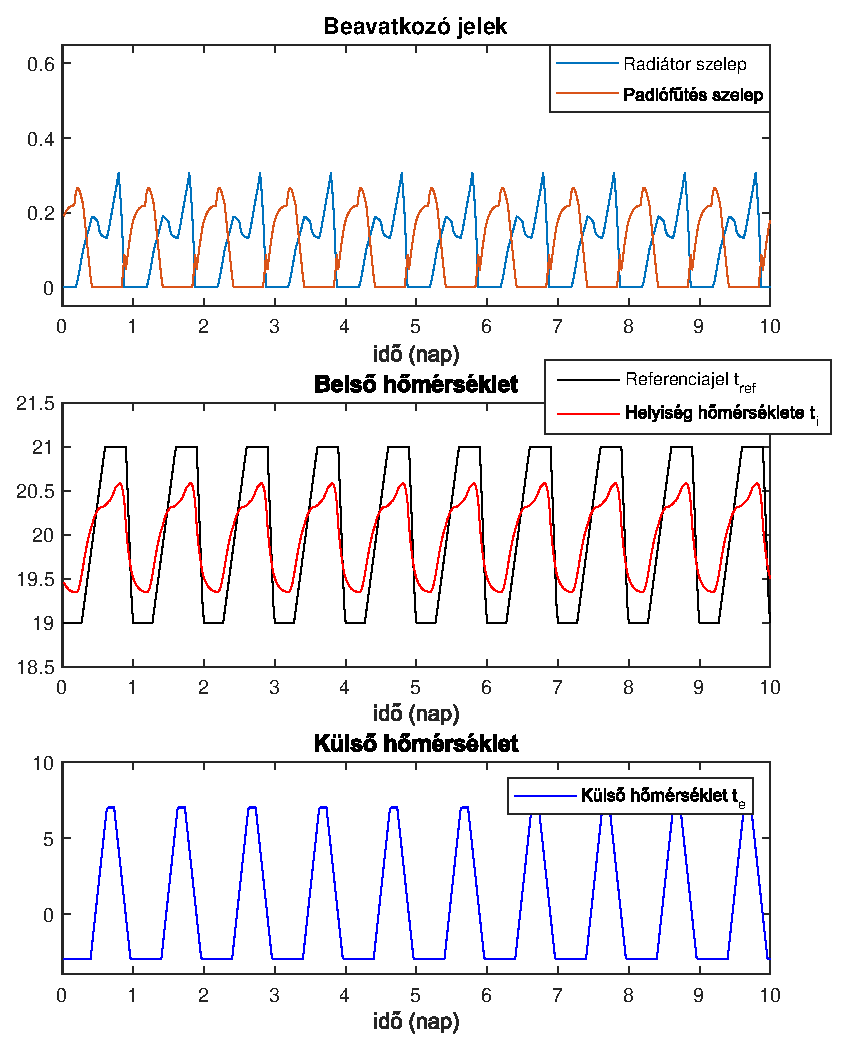
\includegraphics[width=0.35\textwidth, trim=0 0 0 0, clip,]{figures/onlab/Slope/C1Last10ClosedLoop}
	\caption{Referenciajel figyelembe vétele a teljes horizontra C1Last10ClosedLoop}
	\label{fig:onlab-refslprev2}
\end{figure}

\begin{figure}[H]
	\centering
	% trim={<left> <lower> <right> <upper>}
	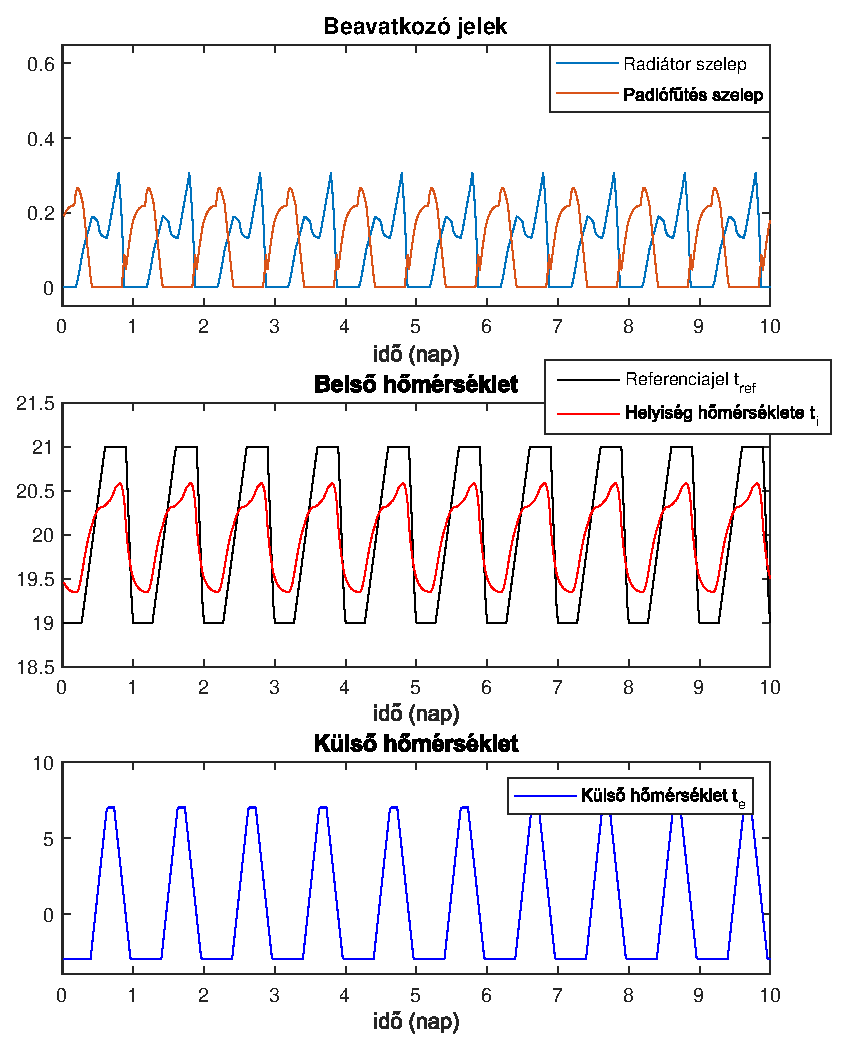
\includegraphics[width=0.35\textwidth, trim=0 0 0 0, clip,]{figures/onlab/Slope/C2Last10ClosedLoop}
	\caption{Referenciajel figyelembe vétele a teljes horizontra C2Last10ClosedLoop}
	\label{fig:onlab-refslprev3}
\end{figure}

\begin{figure}[H]
	\centering
	% trim={<left> <lower> <right> <upper>}
	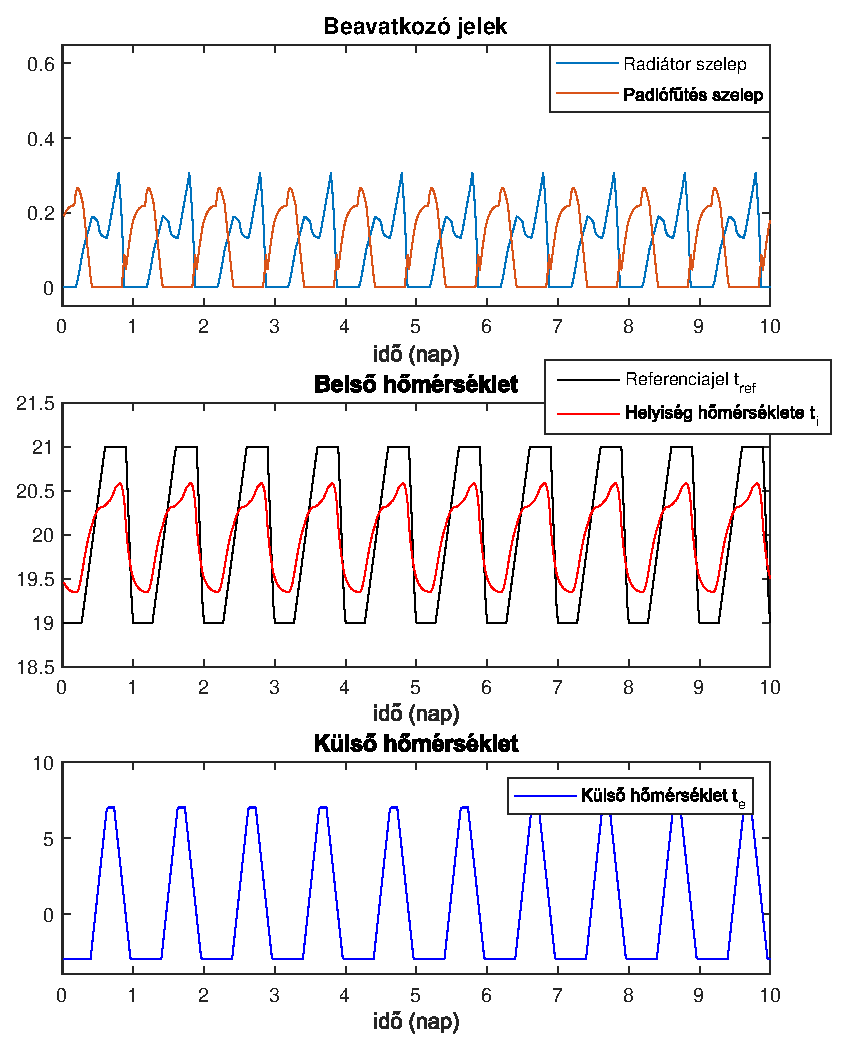
\includegraphics[width=0.35\textwidth, trim=0 0 0 0, clip,]{figures/onlab/Slope/C4Last10ClosedLoop}
	\caption{Referenciajel figyelembe vétele a teljes horizontra C4Last10ClosedLoop}
	\label{fig:onlab-refslprev4}
\end{figure}

\begin{figure}[H]
	\centering
	% trim={<left> <lower> <right> <upper>}
	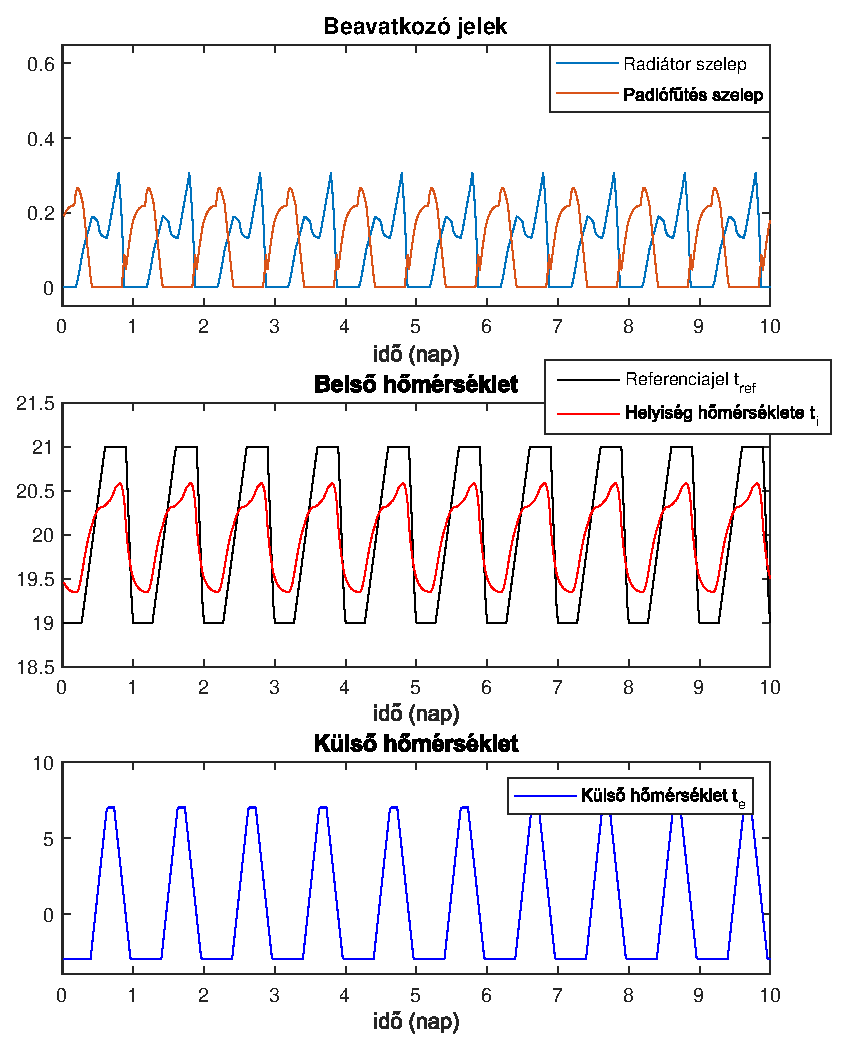
\includegraphics[width=0.35\textwidth, trim=0 0 0 0, clip,]{figures/onlab/Slope/C5Last10ClosedLoop}
	\caption{Referenciajel figyelembe vétele a teljes horizontra C5Last10ClosedLoop}
	\label{fig:onlab-refslprev5}
\end{figure}

\subsection{Összehasonlítás}
\begin{figure}[H]
	\centering
	% trim={<left> <lower> <right> <upper>}
	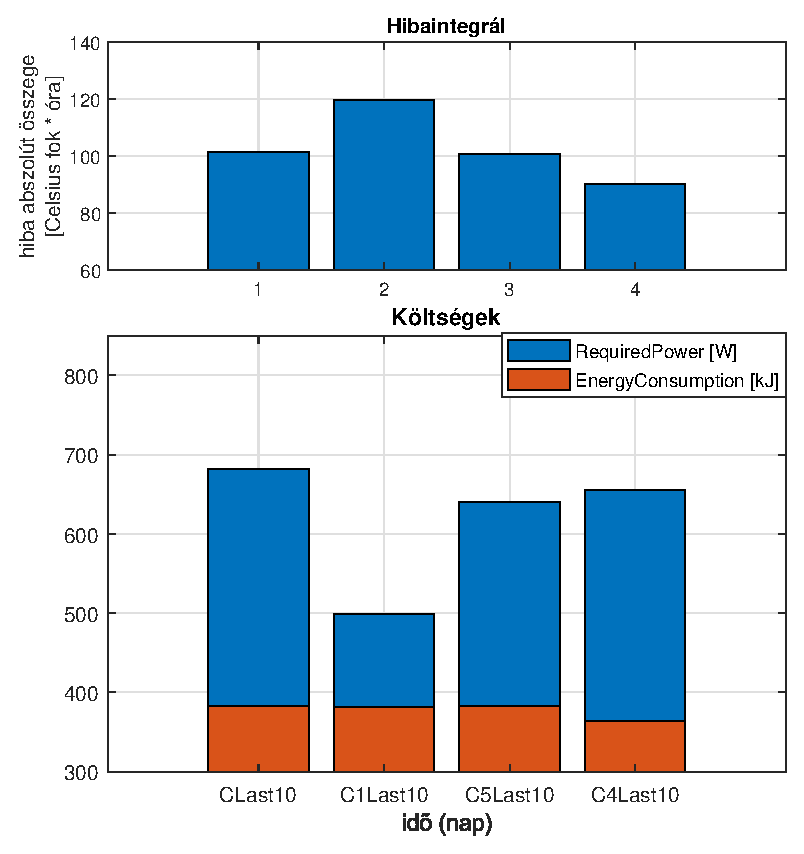
\includegraphics[width=0.35\textwidth, trim=0 0 0 0, clip,]{figures/onlab/Slope/compareControllerPreviewSlope}
	\caption{compareControllerPreviewSlope}
	\label{fig:onlab-refSlprevComp}
\end{figure}


\pagebreak
